\documentclass[UTF8]{ctexart}


\usepackage{picinpar, graphicx} % 导入这个库后,就能支持插入表格
\graphicspath {{img_math/},{img2/}} %图片目录在当前目录的 img 和 img2文件夹下

\usepackage{algorithm, algorithmic, amsmath, amssymb,bm} % 支持数学公式输入
% \usepackage[fleqn]{amsmath} % 公式左对齐

\usepackage{ctex} % 支持字体加粗效果, 代码为 \textbf{加粗}


\usepackage{multicol} %用于实现在同一页中实现不同的分栏
\usepackage{wrapfig} %用于实现图文混排
\setlength{\parindent}{0pt} % 放在段首,之后的所有段落都将取消首行缩进

% 页面边距设置
\usepackage{geometry} %导入版面设置的宏包
\geometry{left=1.5cm, right=1.5cm, top=2cm, bottom=2cm} % 使用命令:\geometry{left=左边距,right=右边距,top=上边距,bottom=下边距}

\usepackage[skins]{tcolorbox} % 导入该包, 才能支持彩色文本框效果.  必须标注skin,才能使用shadow命令显示阴影

\usepackage{soul} % 支持英文高亮
\usepackage{xcolor} 
\newcommand{\mathcolorbox}[2]{\colorbox{#1}{$\displaystyle #2$}}





\title{函数}




%------------------------------------------------------------



\begin{document}
	\tableofcontents % 生成目录
	\maketitle  %这行代码, 让你前面的 title, author, date生效

\part{数列的极限}

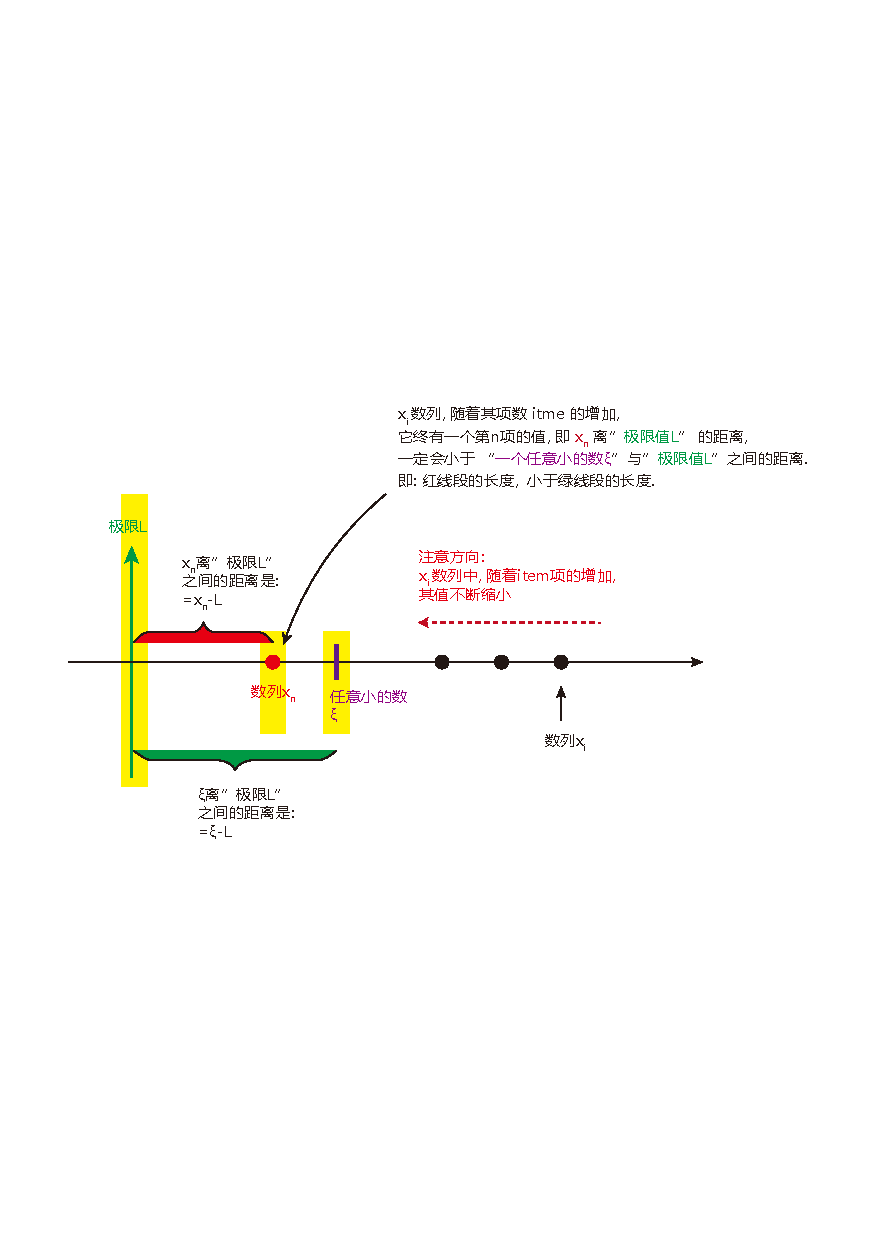
\includegraphics[width=0.7\textwidth]{/0001.pdf}

即: 给定①任意一个极小值ε, ②一个确定的极限值L, ③一个数列 $ x_i $(里面的元素值不断变小). → 则随着数列 
$ x_i $ 中item的增长, 必定会有一个 item项(比如第n项), 该``item项的值 $ x_n$"与``极限值L"的距离, 必定会小于 ``极小值ε"与``极限值L"之间的距离 (这个距离其实就是ε本身). \\



\begin{tcolorbox}[title = {例},boxrule={0.1em},colframe={black!10}, colback={black!3},colbacktitle={black!10},coltitle={black}]
	有数列 $x_n=\dfrac{(-1)^n} {(n+1)^2} $  的极限是0.  问: 该数列取到哪一项item 时, 它与``极限0"之间的距离, 就小于``任意小的数ε"了呢?
	
	即, 问的就是: 该数列与 0 之间的距离, 要小于ε.
	
	
	\[
		\begin{matrix}
			\left| \text{数列}\dfrac{\left( -1 \right) ^n}{\left( n+1 \right) ^2}-\text{极限值}0 \right|<\varepsilon\\
			\left| \dfrac{1}{\left( n+1 \right) ^2} \right|<\varepsilon\\
			\left( n+1 \right) ^2>\dfrac{1}{\varepsilon}\\
			n+1>\dfrac{1}{\sqrt{\varepsilon}}\\
			n>\dfrac{1}{\sqrt{\varepsilon}}-1\\
		\end{matrix}
	\]
	
	为了保证n 为正数(而非有小数点), n就取 $\left( \dfrac{1}{\sqrt{\varepsilon}}-1 \right) +1$	
\end{tcolorbox}



~\\
\hrule
~\\


\part{函数的极限}

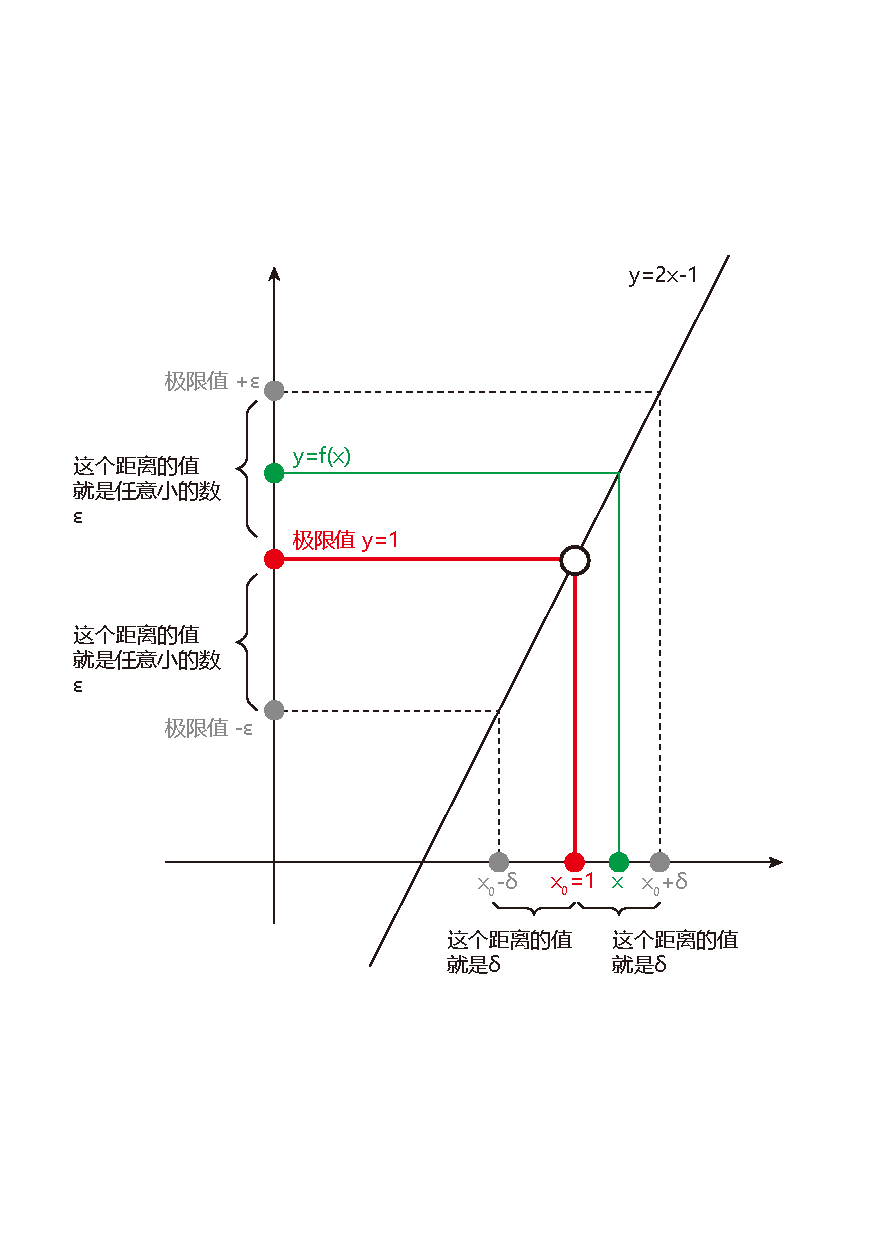
\includegraphics[width=0.5\textwidth]{/0002.pdf}

~\\
\hrule
~\\



\part{极限运算法则}

$ \lim (x \pm y) = \lim x \pm \lim y $ \\
$ \lim (x \cdot y) = \lim x \cdot \lim y $  \\
\\
$ \lim (\dfrac{x} {y}) = \dfrac{\lim x} {\lim y} $ \\
$ \lim (\text{常数} C \cdot y) = \text{常数} C \cdot \lim y $ \\
\\
$ \lim y^n = (\lim y)^n $ \\
$ \lim y^{\frac{1} {n}} = (\lim y)^{\frac{1} {n}} $ \\
\\
$ \lim(\text{常数}C) = \text{常数}C $
\\


\section{若 $ f(x) \textgreater g(x) $, 则 $ \lim f(x) \geq \lim g(x)$  ← 注意: 是大于等于 ≥ !}

这个定理也就是说: 虽然 一个函数, 可能大于另一个函数, 但它们的极限, 是有可能相等的. \\

\begin{tcolorbox}[title = {例},boxrule={0.1em},colframe={black!10}, colback={black!3},colbacktitle={black!10},coltitle={black}]
	虽然 $ \dfrac{1} {x} \textgreater \dfrac{1} {x^2}$, 但它们的极限(在 x → ∞ 时), 却是相等的.  即 $ \lim_{n\rightarrow \infty}\dfrac{1}{x}=\lim_{n\rightarrow \infty}\dfrac{1}{x^2}=0
	$ 
	\\
	
	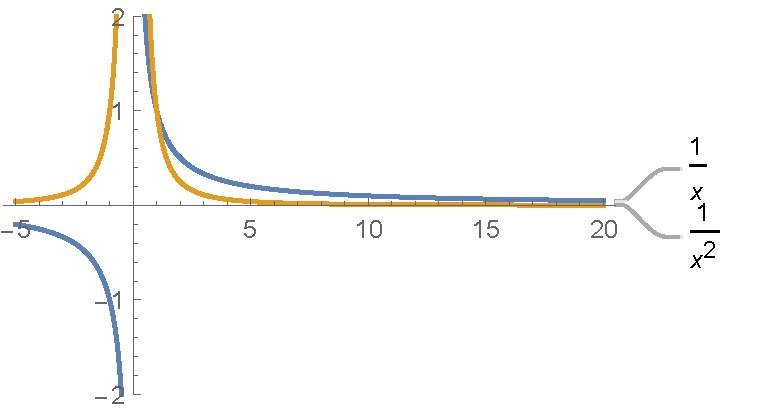
\includegraphics[width=0.4\textwidth]{/0003.pdf}
\end{tcolorbox}



~\\
\hrule
~\\


\part{极限的规律}

\section{分子上``项的最高次数" \textgreater 分母上``项的最高次数", 则 该分式的极限= ∞. 反之, 则极限=0}

一个函数若是``分数" $ \dfrac{a \cdot x^m}{b \cdot x^n} $, 则其极限, 只看它分子分母上的``最高次数"的情况:






\subsection{对于 $ \dfrac{a \cdot x^m}{b \cdot x^n} $, 若 m \textgreater n, 即: 分子的值 \textgreater 分母的值. 则函数极限值 = ∞}






\subsection{对于 $ \dfrac{a \cdot x^m}{b \cdot x^n} $, 若 m=n, 则函数极限值 = $ \dfrac{a} {b}$}

\begin{tcolorbox}[title = {例},boxrule={0.1em},colframe={black!10}, colback={black!3},colbacktitle={black!10},coltitle={black}]
	\begin{align*}  % 支持每行编号. 若不需要编号, 就用 align*环境
			\lim_{x\rightarrow \infty}\frac{3x^3+4x^2+2}{7x^3+5x^2-3}=\underset{\text{把分子分母,\ 同时除以最高项的}x^3}{\underbrace{\lim_{x\rightarrow \infty}\frac{\frac{3x^3+4x^2+2}{x^3}}{\frac{7x^3+5x^2-3}{x^3}}}}=\underset{\text{把}x\rightarrow \infty \text{代入每一项中}}{\underbrace{\lim_{x\rightarrow \infty}\frac{3+\frac{4}{x}+\frac{2}{x^3}}{7+\frac{5}{x}-\frac{3}{x^3}}}}=\frac{3+0-0}{7-0+0}=\frac{3}{7}\\
		\end{align*}
	
	规律: 当满足 ①  $x \rightarrow \infty$, ② 分子分母的最高次的次数相同, 比如本例最高都是 $x^3$ 次, 则: 极限值, 就取分子分母最高次的系数之比. 如 本例就取 $\dfrac{3 x^3} {7 x^3}$ 的系数, 即 $3/7$ , 这个就是极限值了.
\end{tcolorbox}




\subsection{对于 $ \dfrac{a \cdot x^m}{b \cdot x^n} $, 若 n \textgreater m, 即: 分子的值 \textless 分母的值. 则函数极限值=0}

\begin{tcolorbox}[title = {例},boxrule={0.1em},colframe={black!10}, colback={black!3},colbacktitle={black!10},coltitle={black}]
	\begin{align*}  % 支持每行编号. 若不需要编号, 就用 align*环境
			\lim_{x\rightarrow \infty}\frac{3x^2-2x-1}{2x^3-x^2+5}=\underset{\text{把分子分母,\ 同时除以最高项的}x^3}{\underbrace{\lim_{x\rightarrow \infty}\frac{\frac{3x^2-2x-1}{x^3}}{\frac{2x^3-x^2+5}{x^3}}}}=\underset{\text{把}x\rightarrow \infty \text{代入每一项中}}{\underbrace{\lim_{x\rightarrow \infty}\frac{\frac{3}{x}+\frac{2}{x^2}-\frac{1}{x^3}}{2-\frac{1}{x}+\frac{5}{x^3}}}}=\frac{0+0-0}{2-0+0}=0\\
	\end{align*}

	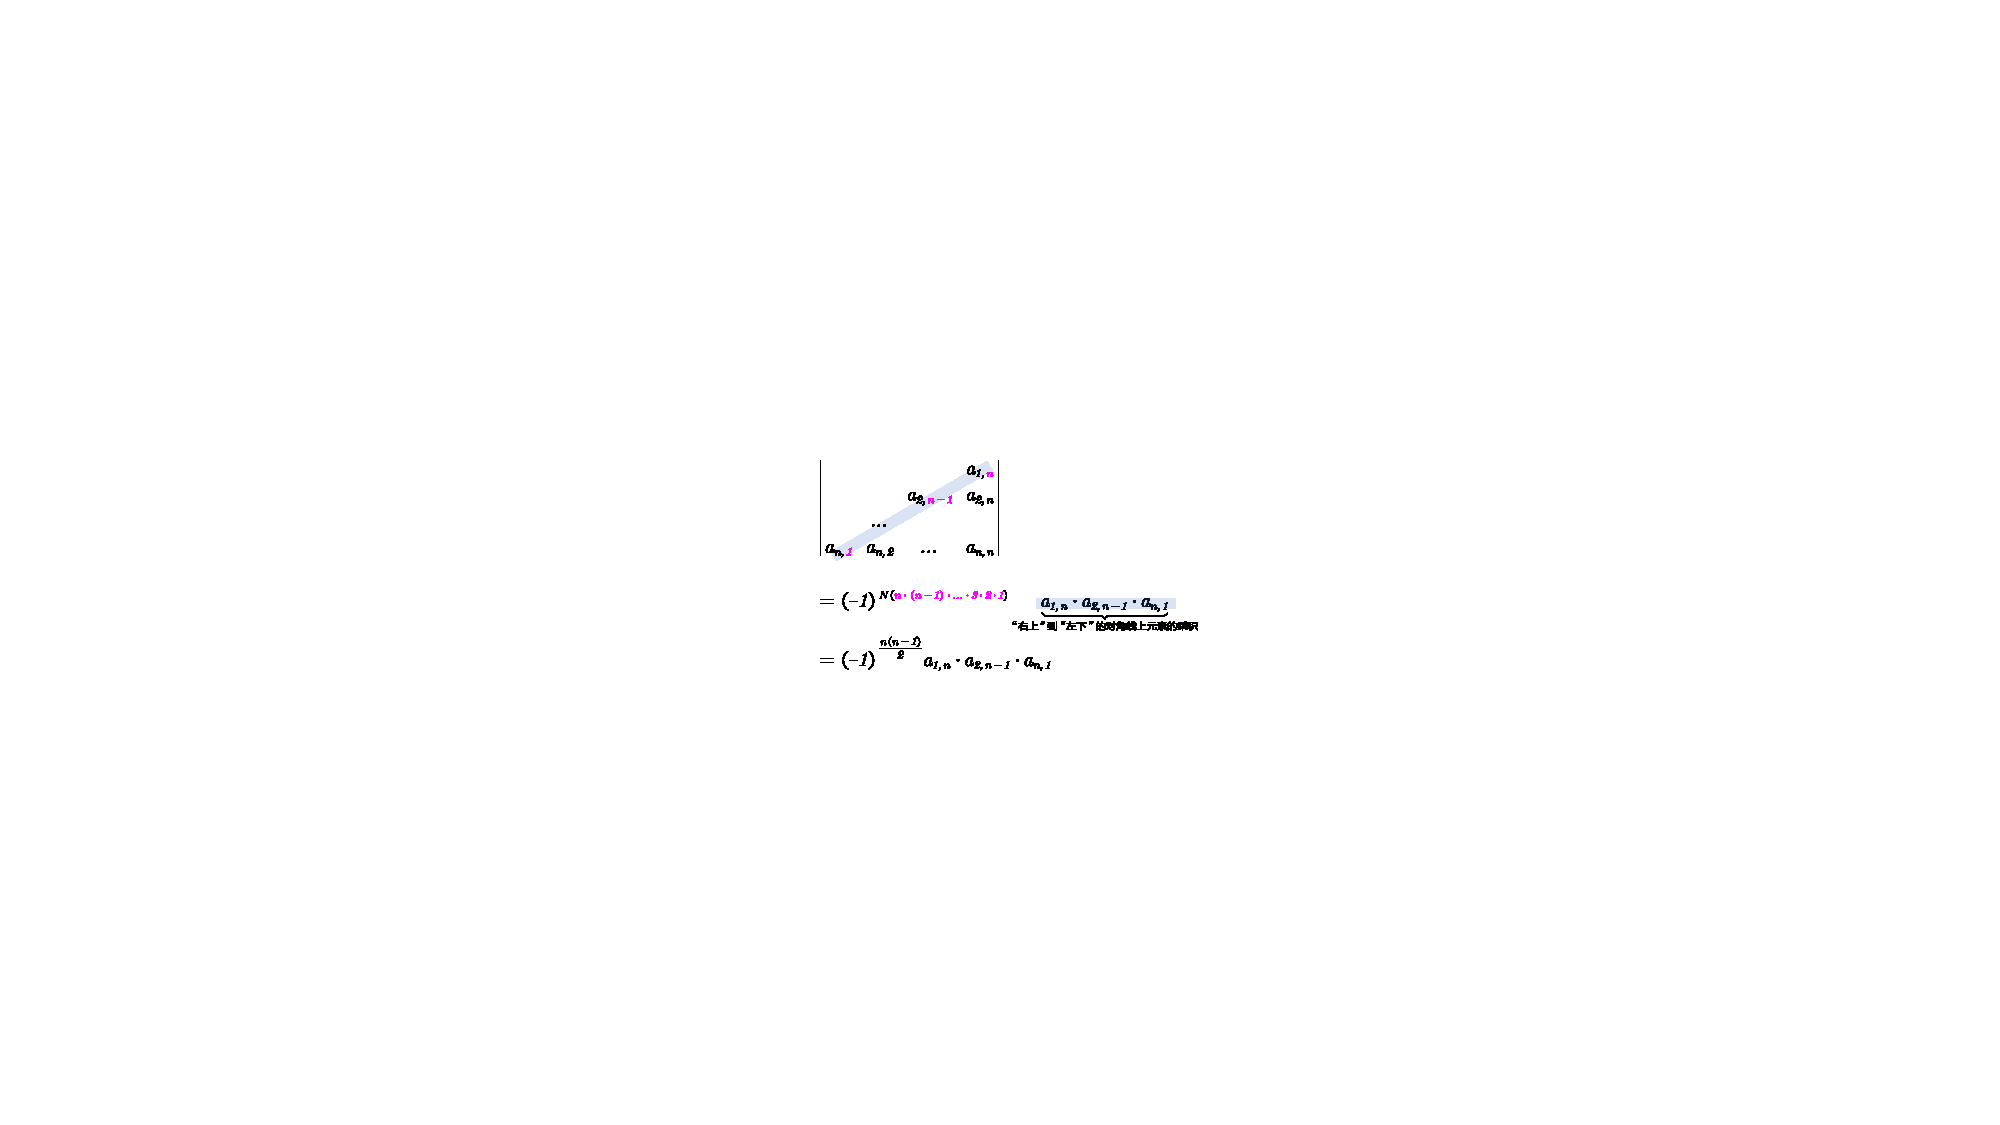
\includegraphics[width=0.4\textwidth]{/0004.pdf}
	
	规律: 当满足 ① $x \rightarrow \infty$, ②分母的最高次的次数, 要比分子的最高次次数还大时, 比如本例``分母的最高次次数"是 $x^3$, 而``分子的最高次次数"只有 $x^2$, 则: 极限就是0.
\end{tcolorbox}


~\\
\hrule
~\\


\part{几个重要的极限}


\section{$ \lim_{x \to 0} \dfrac{\sin x} {x} = 1 $}

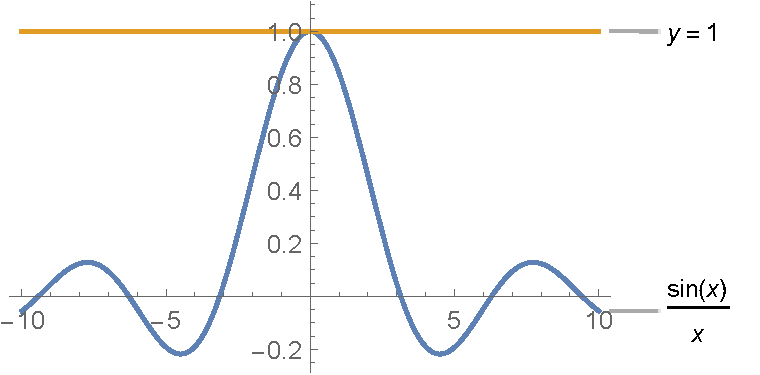
\includegraphics[width=0.4\textwidth]{/0005.pdf}

其实, 它的骨架本质, 是这种形式的: \hl{$\lim_{\Box \to 0} \dfrac{sin \Box} {\Box}$}






\section{$ \lim_{x \to \infty} (1+ \dfrac{1} {x})^x = e $}

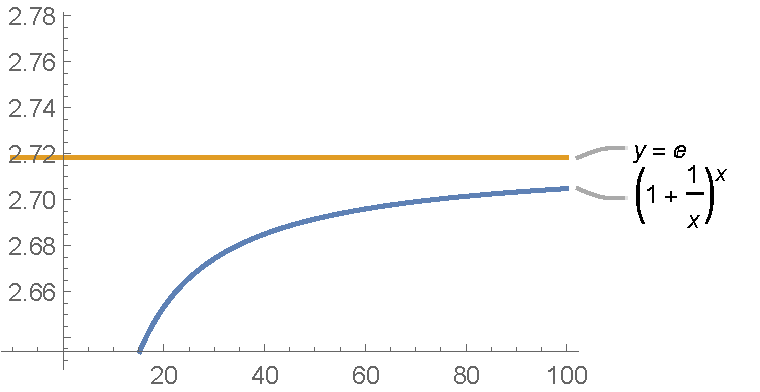
\includegraphics[width=0.4\textwidth]{/0006.pdf}

这个公式其实就是``复利"的终值计算公式: $ \lim_{n \to \infty} (1+ \dfrac{1} {n})^n = e \approx 2.71828 $

注意: 该公式的本质是: \hl{$\lim_{n \to \infty} (1+ \dfrac{1} {\Box})^\Box = e$}.  ← 即两个"方框□"处的数字必须完全相同!

注意: 使用该极限公式时, 中间必须是加号+. 如果题目给出的不是加号, 你也要把它先变换成加号.
	
即: 

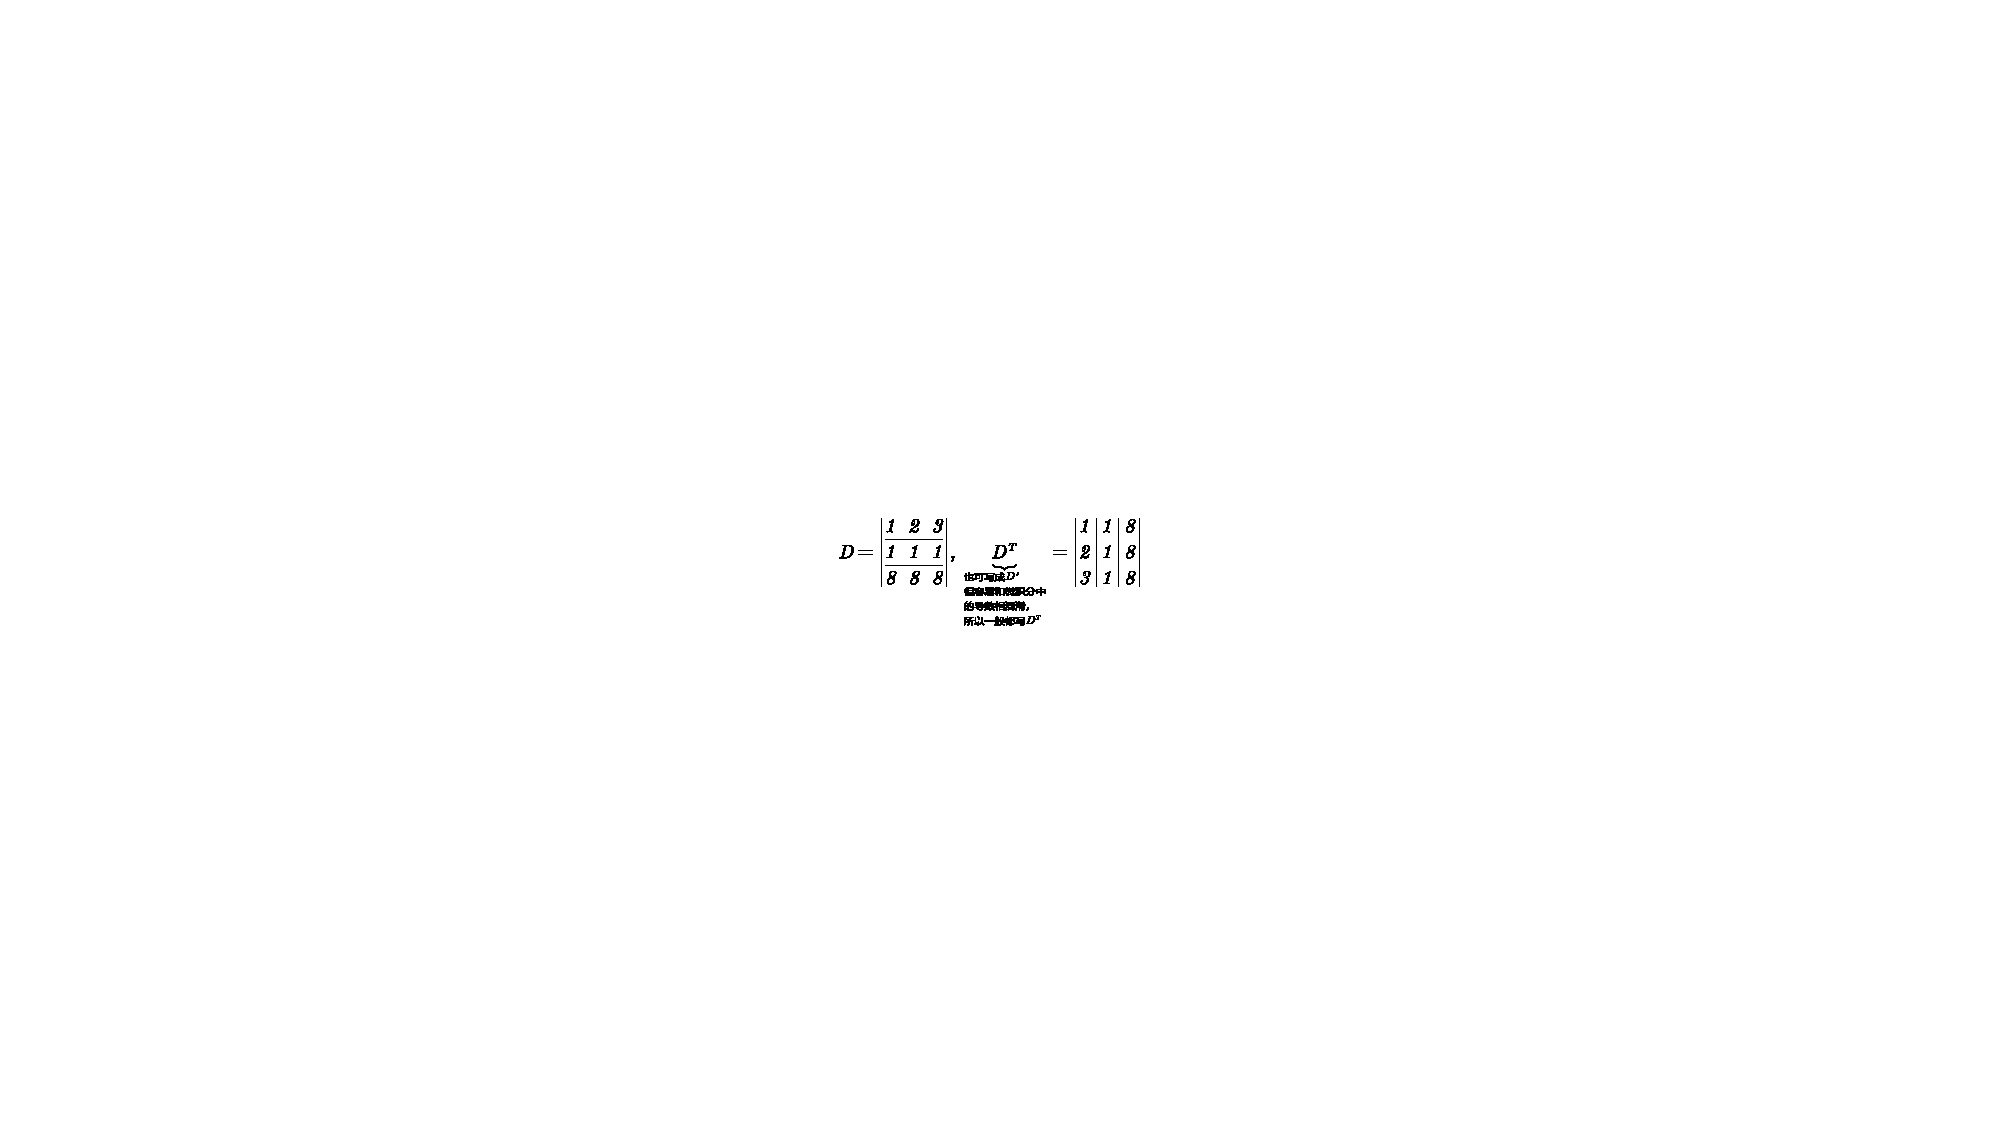
\includegraphics[width=0.25\textwidth]{/0007.pdf}


\section{$\lim_{x \to 0} (1+x)^{\frac{1} {x}} =e $}







\end{document}

